\documentclass[a4paper, 11pt]{article}
\usepackage[utf8]{inputenc}
\usepackage[T1]{fontenc}

% aptitude install texlive-fonts-extra
\usepackage{newcent}

% aptitude install texlive-lang-spanish
\usepackage[catalan]{babel}

\usepackage{amsmath}
\usepackage[pdftex]{color,graphicx}
\usepackage{makeidx}
\usepackage{amssymb}
\usepackage{amsmath}
\usepackage{url}
\usepackage{hyperref}
\usepackage{textcomp}
\usepackage{sverb}
\usepackage[format=plain,labelfont=bf,up,textfont=it,up]{caption}
\usepackage[kerning,spacing]{microtype}
\microtypecontext{spacing=nonfrench}
\usepackage{indentfirst}


% http://stackoverflow.com/questions/1966425/source-code-highlighting-in-latex
% paquet per resaltat de sintaxi
\usepackage{minted}
\newcommand{\pycode}[1]{
  \inputminted[linenos, frame=lines, fontsize=\small]{python}{../#1.py}
}


%opening
\title{Pràctica 1, agent ascensor}
\author{
  Martí Amengual Torrens \small{<marti.amengual.torrens@gmail.com>}, \\
  Pau Ru\l.lan Ferragut \small{<paurullan@gmail.com>}
}

\begin{document}

\maketitle

\thispagestyle{empty}

\begin{abstract}
La insta\lgem ació d'un ascensor que no respongui sols als estímuls mecànics
sinó que decideixi un comportament òptim és una bona iniciació a l'estudi dels
agents inte\lgem igents. En aquesta pràctica es duu a terme l'avaluació de les
clàusules que determinen com un ascensor es comportarà de manera que els seus
ocupants tinguin el millor servei possible. Es proposa una implementació en un
llenguatge de caràcter general i una interfície gràfica amigable.
\end{abstract}

\newpage

\tableofcontents

\newpage

\section{Introducció}

Consideris el cas d'un ascensor senzill que pot percebre la següent informació
del seu entorn:

\begin{itemize}
  \item En quin pis es troba aturat.
  \item A quins pisos volen anar els ocupants.
  \item En quins pisos hi ha persones que volen entrar a l'ascensor. Es
    considera que hi ha dos botons per cridar l'ascensor, un de pujada i un de
    baixada.
  \item L'estat de la porta (oberta o tancada).
\end{itemize}

A més, l'ascensor es capaç de realitzar les següents accions:

\begin{enumerate}
  \item Pujar un pis, a no ser que estigui al darrer pis.
  \item Baixar un pis, a no ser que estigui a la planta baixa.
  \item Obrir la porta.
  \item Tancar la porta.
  \item Esperar $\delta$ segons per tal que els usuaris puguin entrar i sortir.
\end{enumerate} 

Amb aquestes dades s'ha de dissenyar un agent capaç de controlar l'ascensor de
forma eficient. No serà eficient, per exemple, canviar el sentit de l'ascensor
quan estigui pujant si encara hi ha algú adins que vol pujar a un pis superior
o si hi ha algú a fora que hagi so\lgem icitat entrar a l'ascensor des d'algun
pis superior.

\section{Avaluació del problema}

Per tal de resoldre la pràctica hem dissenyat un agent estímul-resposta (d'ara
endavant \emph{agent ER}) amb estat intern. L'agent rep unes percepcions de
l'ambient, on a partir d'aquets estímuls i el seu estat intern és capaç
d'escollir l'acció més eficient.

Per tal de que l'agent ascensor sigui eficient no ha estat suficient resoldre'l
a través d'un simple agent ER sinó que hem hagut d'afegir un estat intern.
Aquesta informació ajudarà a l'agent a decidir quina acció toca executar per
tal de satisfer les necessitats dels usuaris. A més, amb l'estat intern, se'ns
permetrà fer-ho minimitzar els canvis de sentit per així proporcionar la millor
experiència possible als usuaris.

A continuació es descriuen amb més detall cada una d'aquestes característiques
enunciades: percepcions, accions, estat intern, estat de l'ambient.

\subsection{Percepcions}

Les percepcions de l'agent ascensor són les senyals o estímuls que percep de
l'ambient on treballa. El nostre agent ascensor podrà percebre:

\begin{itemize}
  \item El pis on es troba situat.
  \item Una llista de les peticions de sortida de les persones que es troben a 
  l'interior.
  \item Una llista de les peticions d'entrada per tal de pujar de pis.
  \item Una llista de les peticions d'entrada per tal de baixar de pis.
  \item Si la porta està oberta o tancada.
\end{itemize}

Si analitzam les percepcions podem deduir que l'ascensor només podrà canviar de
pis mentre la porta estigui tancada. Si la porta esta oberta l'agent ascensor
no podrà pujar ni baixar de pis. Com que en tot moment l'agent sap en quin pis
esta situat podrà deduir fàcilment quin tipus de peticions té dels pisos
superiors i inferiors.

El problema ve de que aquestes percepcions no proporcionen suficient informació
com per decidir l'acció i necessitam saber les darreres accions i moviments de
l'ascensor. Per aquest motiu s'utilitza un estat intern que es descriu en el
proper subapartat.

\subsection{Estat intern}

Com s'ha mencionat abans, únicament amb les percepcions no es suficient decidir
quina acció convé aplicar l'agent ja que podrà ser diferent depenent de si
l'ascensor es trobà en sentit de pujada o baixada. Per aquest motiu hem definit
un estat intern caracteritzat pel sentit de l'ascensor (pujada o baixada) i per
l'última acció realitzada.

No ens es suficient que l'estat intern sigui exclusivament la darrera acció
realitzada per l'agent perquè aquesta no es pot determinar el sentit del
mateix.  Per exemple, en el cas que en algun determinat pis l'ascensor s'ha de
parar per obrir la porta, esperar $\delta$ segons i tancar la porta, l'última
acció de tancar la porta, no ens determina si l'ascensor estava baixant o
pujant de pis.  Com que no ho sabem l'ascensor podria actuar de manera
ineficient. Per tant, hem de saber en tot moment amb quin sentit es troba
l'ascensor.

\subsection{Accions}

Explicant les percepcions i l'estat intern de l'agent gairebé ja hem definit
les accions de l'ascensor. En tot cas les accions que pot escollir l'agent són
aquestes cinc:

\begin{enumerate}
  \item Pujar un pis, a no ser que l'ascensor estigui al darrer pis.
  \item Baixar un pis, a no ser que l'ascensor estigui a la planta baixa.
  \item Obrir la porta.
  \item Tancar la porta.
  \item Esperar $\delta$ segons per tal de que els usuaris de l'ascensor puguin 
  sortir i entrar de l'ascensor.
\end{enumerate} 

\subsection{Estat de l'ambient}

L'ambient de l'agent ascensor estarà definit per diferents estats. Aquests
estats ho determinaran les diferents combinacions de l'estat de l'ascensor i
les peticions que realitzin els usuaris. L'estat de l'ascensor vendrà
determinat per el pis on es troba l'ascensor i per com es trobin les portes
d'aquest (obertes o tancades). Les peticions que realitzin els usuaris per
sortir o entrar a l'ascensor complementaran el seu estat i d'aquesta manera
definiran els diferents possibles estats de l'ambient.

\section{Regles de l'agent}

Per a definir les regles de l'agent ens ajudarem de les següents funcions/variables:
\begin{itemize}
\item pujada / baixada: representarà el sentit de l'ascensor a través de l'estat intern.
\item esperat\_$\delta$\_segons: representarà si l'última acció ha estat esperar $\delta$ segons per tal de que els usuaris puguin entrar i sortir de l'ascensor.
\item obert / tancat: representarà l'estat de la porta.
\item peticio\_sortida(actual): representarà si hi ha una petició de sortir de l'ascensor en el pis actual.
\item peticio\_pujada(actual): representarà si hi ha una petició de pujar en el pis actual.
\item peticio\_baixada(actual): representarà si hi ha una petició de baixar en el pis actual.
\item peticions\_inferiors: representarà si existeixen peticions als pisos inferiors, tant siguin de sortida, pujada i baixada.
\item peticions\_superiors: representarà si existeixen peticions als pisos superiors, tant siguin de sortida, pujada i baixada.
\end{itemize}

Les regles de l'agent que hem dissenyat són les següents:

\begin{enumerate}
\item obert i esperat\_$\delta$\_segons $\Rightarrow$ tancar
\item obert $\Rightarrow$ esperar\_delta\_segons
\item tancat i peticio\_sortida(actual) $\Rightarrow$ obrir
\item tancat i pujada i peticio\_pujada(actual) $\Rightarrow$ obrir
\item tancat i baixada i peticio\_baixada(actual) $\Rightarrow$ obrir
\item tancat i pujada i peticions\_superiors $\Rightarrow$ pujar
\item tancat i baixada i peticions\_inferiors $\Rightarrow$ baixar
\item tancat i pujada i peticions\_inferiors $\Rightarrow$ baixar
\item tancat i baixada i peticions\_superiors $\Rightarrow$ pujar
\item tancat i pujada i peticio\_baixada(actual) $\Rightarrow$ obrir
\item tancat i baixada i peticio\_pujada(actual) $\Rightarrow$ obrir
\end{enumerate}

\section{Funcionament dels moderns i actuals ascensors}
%http://es.wikipedia.org/wiki/Ascensor
Actualment podem diferenciar dos tipus d'ascensor segons l'algorisme de 
funcionament, un amb un sol botó de cridada exterior a cada pis i un amb dos 
botons de cridada exterior a cada pis; un botó per ascendir de pis i un botó per 
descendir de pis.

Com que l'ascensor dissenyat a la pràctica es a través de dos botons de cridada 
exterior per cada pis, anem a centrar-nos en aquest tipus. L'algorisme que 
utilitzen els ascensors reals segueixen els mateixos principis utilitzats a la 
pràctica per tal de gestionar les peticions internes i externes de l'ascensor. A 
continuació s'exposa el seu mode de funcionament i així podem comprovar que és 
el mateix que el que s'utilitza a la pràctica.

Funcionament en pujada: l'ascensor es va aturant a tots els pisos marcats des de 
l'interior i també en els pisos on hi ha una petició marcada de pujada, però no 
en els que només estigui marcat la petició de baixada. Un cop arribat al pis més 
elevat on hi hagi hagut peticions de pujada es canvia de sentit per tal de 
funcionar en mode baixada.

Funcionament en baixada: l'ascensor es va aturant a tots els pisos marcats des 
de l'interior i també en els pisos on hi ha una petició marcada de baixada, però 
no en els que només estigui marcat la petició de pujada. Un cop arribat al pis 
més inferior on hi hagi hagut alguna petició es canvia de sentit per tal de 
funcionar en mode pujada.

A més, també podem trobar-nos ascensors més complexos formats per més d'una 
unitat. Aquests ascensors tenen un sistema de coordinació. Aquest sistema de 
coordinació processa l'estat de cada unitat de l'ascensor decidint en tot moment 
quina d'ella es més avantatjosa per tal de servir cada petició disminuint així 
el temps d'espera per parts dels usuaris.

Com hem pogut observar, els funcionament dels ascensors reals és el mateix que 
l'utilitzat a la pràctica, treballant d'una manera inte\lgem igent i eficient.

\section{Manual d'usuari}

Un cop arrancada l'aplicació se'ns presentarà una finestra gràfica amb un
conjunt d'accions per dur a terme:

\begin{enumerate}
  \item Anar a un pis des de l'interior de l'ascensor
  \item So\lgem itar pujar des de la planta baixa fins a l'antepenúltim pis
  \item So\lgem itar baixar des del primer fins al darrer pis
  \item Iniciar una demostració de comportament
  \item Tancar l'aplicació 
\end{enumerate}

A la figura \ref{captura1} s'assanyalen els botons distints que es corresponen
a les accions possibles. 

La figura 2 representa l'estat en funcionament del programa. Es pot veure una
interacció, com tenim varis estímuls en marxa i una animació a l'ascensor que
ens indica el seu estat intern.

S'ha adjuntat un petit conjunt de demostracions per facilitar l'avaluació de la
interfície gràfica, automatitzant jocs de prova com un ascensor que puja varis
pisos o un que ha de resoldre una situació de vàries peticions. Aquestes
demostracions són semblants als casos d'ús que es varen usar per verificar el
comportament lògic de l'ascensor. D'aquesta manera l'usuari pot ràpidament
confirmar les possibilitats gràfiques i estudiar apartats com les animacions o
els temps $delta$ d'apertura de portes.

\begin{figure}
\begin{center}
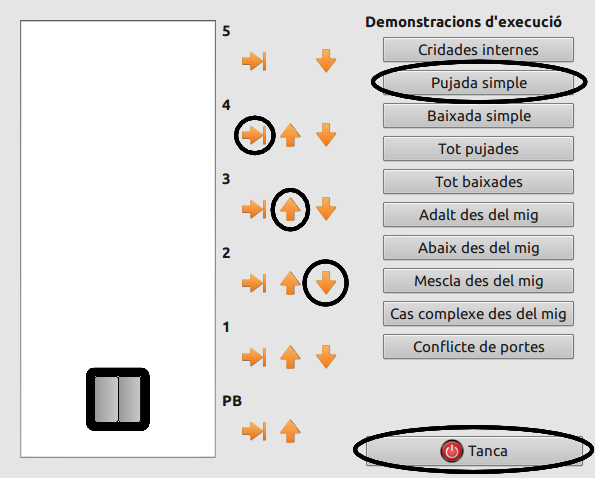
\includegraphics[width=0.8\textwidth]{pantalla-1.png}
\caption{Captura de pantalla de la interfície gràfica}
\label{captura1}
\end{center}
\end{figure}

\begin{figure}
\begin{center}
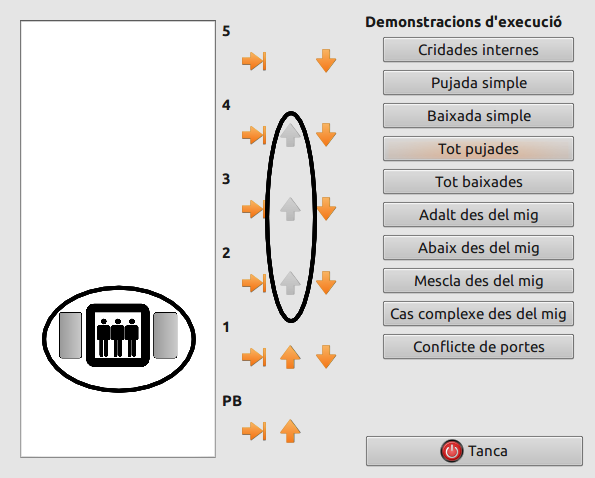
\includegraphics[width=0.8\textwidth]{pantalla-2.png}
\caption{Captura de pantalla de la interfície gràfica}
\label{captura2}
\end{center}
\end{figure}


\newpage
\section{Conclusions}

La pràctica ha sigut tot un repte sobretot en l'aspecte de la
presentació. Malgrat la traducció de les clàusules lògiques i l'esquema de
comportament no va resultar massa complicada la creació d'una interfície
gràfica atractiva ens va portar més hores de les esperades. De tota manera
esperam haver guanyat flexibilitat en aquest aspecte de tal manera que en
futures pràctiques poguem lliurar resultats del mateix nivell de qualitat amb
molt manco temps.




\newpage
\appendix

\section{Implementació}

Per la implementació de la pràctica s'ha optat pel llenguatge de propòsit
general Python i les biblioteques gràfiques QT mitjançant els \emph{bindings}
PyQt4. El disseny de la pràctica s'ha fet de tal manera que tenim quatre
fitxers distints, quadasqun amb els seus objectius concrets:

\begin{description}
   \item[elevator.py] Cos lògic de l'agent ascensor
   \item[test.py] Jocs de proves de l'agent ascensor
   \item[igu.py] Classes de la interfície gràfica
   \item[main.py] Programa principal
\end{description}

\newpage

\addtolength{\hoffset}{-2cm}

\subsubsection*{Agent ascensor - elevator.py}
\pycode{elevator}

\subsubsection*{Jocs de proves lògics - test.py}
\pycode{test}

\subsubsection*{Interfície gràfica - igu.py}
\pycode{igu}

\newpage
\subsubsection*{Programa principal - main.py}
\pycode{main}

\newpage

\addtolength{\hoffset}{2cm}



\end{document}
